\chapter{Zero-Knowledge Proofs}

\section{Definitions}

\subsection*{Proofs}
Intuitively, a \emph{proof} for a statement X is a set of true statements $S_1,S_2,\dots$ which ultimately derive 
from the axioms of the underlying theory and show the statement X to be true. The one who gives the proof 
is said to be the \emph{prover} and the one who "reads" the proof and verifies that it indeed does show the 
desired result is called a \emph{verifier}. We may think of the prover and the verifier as two algorithms 
which take some input and give some output. Here the prover is allowed any amount of computation power but 
usually the constraint is to have the verifier work in polynomial time or perhaps expected polynomial time. \\

\subsection*{Schemes}
\noindent The proof protocol or \emph{scheme} is the entire "interaction" of the prover and the verifier. This 
includes the "behaviour" of the prover and the verifier and any randomness used in the entire process. 
A proof scheme is said to be \emph{complete} if a correct proof gets accepted by the verifier with high 
probability. The counterpart of this property is that a proof scheme is said to be \emph{sound} if an 
incorrect proof gets rejected by the verifier with high probability. Ideally, we would 
like the "high probability" to be 1 but relaxing that criteria is incredibly useful because it 
allows innovative proof schemes which reduce things like memory and time usage!\\

\subsection*{Interactive Proofs}
\noindent An \emph{interactive} proof is a back and forth interaction between the prover and the 
verifier. The verifier asks a question, the prover sends the answer, and the verifier checks if 
the answer is correct. This may be repeated as many times as needed (while keeping the overall verifier run 
time polynomial in its input size). The utility of the interactive proof is that the verifier can ask 
random questions which must be answered "on the fly" -- this is not possible in the one-way method 
of proof in which prover sends a proof to the verifier and verifier can only read the proof. \\

\subsection*{Zero-Knowledge}
\noindent Usually, a proof for a statement reveals some additional information beyond the validity of the statement. 
For example, proving that a number is composite can be given by revealing a factor of the number 
not equal to 1 or the number itself. In this proof, the verifier gains \emph{knowledge} by reading the 
proof, namely a factor of the number which is extra information as compared to only stating compositeness. 
The concept of gaining knowledge can be rigorously defined as not changing the probability distribution over 
something for the verifier but for our purposes the intuitive meaning is enough!\\

\noindent Suppose the prover possesses some secret information and wants to prove to the verifier that they 
indeed possess it without revealing the actual information. A scheme which accomplishes this while being 
sound and complete is called a \emph{zero-knowledge proof}. The term "zero-knowledge" comes from the fact that 
because the verifier gains no knowledge beyond the fact that the prover possesses the secret. This has 
important applications -- if such a proof method exists, it enables two people to verify that 
they indeed share a secret without revealing the secret in case the 
one of them is faking it and should not know the secret. To make these ideas more concrete, we will see some 
examples.\\

\section{Card Color}
Given the standard deck of $52$ cards, a card from the deck has three properties -- color, suit and rank. 
Suppose the prover draws a card from the deck without showing it to anyone. The prover claims that they are 
holding a red card. How can he prove this without revealing the other 2 properties of the card, namely 
suit and rank? Clearly, showing the card to the verifier is not an option since that would reveal the other 
two properties.

So we wish to design a scheme where the prover can prove that they are holding a red card without revealing 
the secret. So at the end of the proof, the verifier should have no idea what card it is among the $26$ red 
cards in a standard deck. 

\subsection{The Scheme}
The prover keeps their card face down separate from the deck. The prover then goes through the remaining deck 
without showing any card to the verifier. The prover puts all cards which are black face up, revealing 
them to the verifier and puts all remaining cards (red) face down, not revealing them to the verifier.
The verifier accepts the proof if the number of black cards revealed is $26$ otherwise the proof is rejected.
\subsection{Completeness and Soundness}
If the prover was indeed holding a red card, then he will be able to reveal $26$ black cards. If the prover 
was lying, they will be able to produce at most $25$ black cards no matter what. The scheme is 
\textbf{complete} because a correct proof will be accepted by the verifier with probability 1. 
The scheme is \textbf{sound} because a incorrect proof will be rejected by the verifier with probability 1.

\section{Graph Isomorphism}
Given two graphs \(G_1\) and \(G_2\), the \emph{graph isomorphism problem} is to determine 
if they are isomorphic. This decision problem is $\NP$ because the answer \texttt{YES} has a polynomially 
verifiable certificate -- the permutation $\sigma$ which converts $G_1$ to $G_2$! The problem is believed 
to not be in $\classP$ since the best algorithm for it is slower than polynomial time.

Let us say there exists an open problem of determining whether two publicly known graphs $G_1$ and $G_2$ 
are isomorphic or not. Now a prover claims to have done the requisite computation 
and found the isomorphism $\sigma$, proving that the graphs are isomorphic. 
To avoid someone stealing the credit for his hard work, he does not want to share the isomorphism 
with the verifier but wants to show that he indeed possesses the secret isomorphism. 

\subsection{The Scheme}

The prover generates a random permutation $r$ and applies it to the vertex labeling of $G_1$. This 
produces a graph $G^*$ which is isomorphic to $G_1$ and of course, is also isomorphic to $G_2$. The prover 
sends $G^*$ to the verifier. The verifier can ask only one of the two following things:

\begin{enumerate}
	\item $Q_1$: What is the permutation that would convert $G_1$ to $G^*$? ($r$)
	\item $Q_2$: What is the permutation that would convert $G^*$ to $G_2$? ($\sigma \circ r^{-1}$)
\end{enumerate}

\vspace{0.5em}
\begin{center}
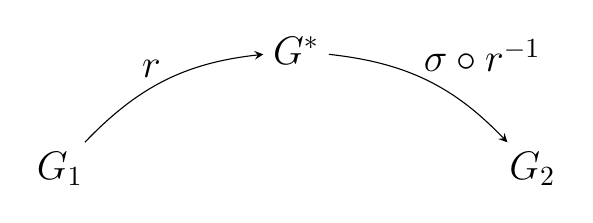
\begin{tikzpicture}[every node/.style={font=\Large},>=stealth]
\node (G1) at (0,0) {$G_1$};
\node (Gs) at (3,1.5) {$G^*$};
\node (G2) at (6,0) {$G_2$};

\draw[->]
(G1) to[bend left=20]
node[midway,xshift=-5pt, yshift=4pt] {$r$}
(Gs);

\draw[->]
(Gs) to[bend left=20]
node[midway,xshift=20pt, yshift=9pt] {$\sigma \circ r^{-1}$}
(G2);

\end{tikzpicture}
\end{center}

The verifier asks $Q_1$ and $Q_2$ with equal probability and verify the answer. If answer is 
correct, the verifier accepts otherwise declines.

\subsection{Soundness and Completeness}
If the prover truly knows the secret, he will be able to answer any one of $Q_1$ and $Q_2$ correctly because 
he knows $r$ and $\sigma$ so he will be able to calculate $\sigma \circ r^{-1}$. But if he is a faker and he 
created $G^*$ by doing $G_1 \circ r$, then he will only be able to answer $Q_1$ correctly and fail 
to answer $Q_2$ since he doesn't know $\sigma$. Similarly if he fakes $G^*$ by doing a random $G_2 \circ r$ 
then he won't be able to tell how to permute $G^*$ to get $G_1$.\\ 

For an actual prover, we will run this scheme $k$ times and since the answer will be correct, we will 
accept with probability 1. Thus the scheme is \textbf{sound} because we accept a correct proof with high 
probability.\\

For a faker, the probability of being able to answer a random question among $Q_1$ and $Q_2$ correctly is 
at most $\frac{1}{2} + \frac{1}{2} \cdot \frac{1}{|V|!-1}$. This is because there is a $\frac{1}{2}$ probability of getting 
the question which he "prepared" for and if he gets the other question, then he can answer a random permutation 
which is not the inverse of the one he prepared (because $G_1 \ne G_2$) -- there are $|V|!-1$ such permutations. Since the 
second term is quite small for even $|V| \ge 10$ also, it doesn't really matter so usually 
it is dropped and we say that the faker always gets caught when it is the other question.

Thus a faker will be rejected with probability $1-\frac{1}{2^k}$ for $k$ independent runs of 
this scheme. Since in polynomial time we can run this scheme any $k$ times, we can achieve as high a 
probability of rejection as we want. Thus the scheme is \textbf{sound}!

In general for soundness we can put the condition that if input size is $n$ then rejection of incorrect proof 
should be done with probability at least $\frac{1}{n^c}$, where $c>0$ because we can run the scheme 
independently a polynomial number of times to make it as high a probability of rejection as we want. 

Interestingly, this scheme can be viewed intuitively as a $\coRP$ decision problem from the perspective of 
the verifier -- the verifier says \texttt{YES} if the proof is correct and \texttt{NO} if the proof is 
incorrect. The verifier always says \texttt{YES} when the actual answer is \texttt{YES} and says 
\texttt{NO} when the actual answer is \texttt{NO} with probability at least $\frac{1}{n^c}$. Indeed, 
the definition has $\frac{1}{n^c}$ as a lower bound because of the exact same reason as here -- we must be 
able to achieve any high probability of being correct by running this scheme a polynomial number of times.

\subsection{Game Theory Perspective}
Let $|V|=n$ be the number of vertices in the graph $G_1$. An interesting perspective on this scheme is 
looking at it as a two-player game between the faker and the verifier. 

The faker has two actions $A_1$ and $A_2$ -- he can fake $G^*$ by doing $A_1$ which is $G_1 \circ r$ or 
$A_2$ which is $G_2 \circ r$. The verifier has two actions $Q_1$ and $Q_2$ -- the two questions. The game 
has both of them choosing only one of the actions. The game is a zero-sum game with payoff matrix is 
as follows:

\[
\begin{tabular}{|c|c|c|}
\hline
\diagbox {$S_V$}{$S_F$} & $A_1$ & $A_2$ \\
\hline
$Q_1$ & (-1,1) & (1,-1) \\
\hline
$Q_2$ & (1,-1) & (-1,1) \\
\hline
\end{tabular}
\]

Notice this is the exact same game as the penalty-kick game we saw in the chapter on game theory. So 
we recall there existed a mixed strategy Nash equilibrium with both players choosing each action with 
equal probability and the expected payoff is 0. Since the optimal play from verifier is to ask $Q_1$ and 
$Q_2$ with equal probability, we can guarantee a payoff of at least 0 in our scheme since the 
verifier plays optimally. Let $p_{\text{catch}}$ be the probability of catching the faker.

\[
\mathbb E[U_V] =  p_{\text{catch}} \cdot (1) + (1-p_{\text{catch}}) \cdot (-1) \ge 0
\]

\[
\implies 
2p_{\text{catch}}-1 \ge 0
\implies 
p_{\text{catch}} \ge \frac{1}{2}
\]

